%=====================================================================
\section{Introduction}
\label{sec:intro}
Real networks evolve: nodes and links appear and disappear, and interactions take
place at specific moments---a conversation lasts a minute, a message is sent at a
given second, a paper cites earlier work in a given year. Classical network analysis
nevertheless collapses all of this into one static graph in which two nodes are either
linked or not. Such aggregation is convenient, but it discards when links are active,
how often they recur, in which order they occur and how the network changes. Unlike
for static graphs, connectedness is not transitive in time, so a temporal network cannot
be reduced to a simple graph without loss \citep{holme2015modern}. The
temporal-network literature \citep{holme2012temporal,holme2015modern,masuda2016guide}
has shown that each of these ingredients can change the conclusions drawn about
structure, communities, and processes such as epidemics.

Most of this evidence, however, comes from a single dataset or a single method. It
is therefore hard to tell \emph{how much} time matters in general, and for which kinds
of systems. We address two research questions.
\textbf{RQ1:} how does temporal information change our understanding of the structure
and function of real networks, and how does this effect differ across network types?
\textbf{RQ2:} which hypotheses from the temporal-network literature (H1--H7,
\cref{tab:hypotheses}) hold in which systems?

\paragraph{Approach.}
The report is organised around four questions that recur in every section
(\cref{fig:framework}): (I) \emph{representation}---what is lost by aggregation and
by the choice of time window? (II) \emph{activity patterns}---are interactions bursty,
repeated and persistent? (III) \emph{structural evolution}---how do networks grow,
age and reorganise? (IV) \emph{function}---does time ordering change reachability,
centrality and spreading? Each question is turned into a literature hypothesis, a
metric and a randomized reference model \citep{gauvin2022randomized}, and applied to
three networks that differ in edge meaning, generating mechanism and time scale
(seconds, seconds, years): face-to-face contacts, online messages and citations.
Because raw metrics are not comparable across such systems, datasets are compared via
\emph{normalised time effects} (\cref{sec:time-effect}). We do not propose new
models; the contribution lies in the common framework and the comparison.

\begin{figure*}[t]
\centering
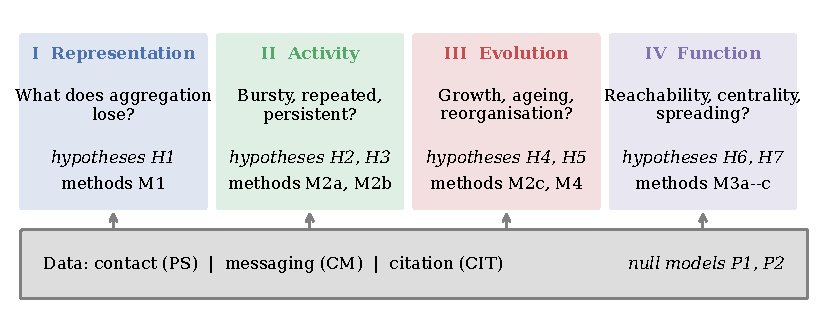
\includegraphics[width=\textwidth]{fig_framework.pdf}
\caption{Structure of the study. Four questions (Parts I--IV) map to seven
hypotheses and four method groups; the same order is used in Related Work, Methods,
Results and Discussion. All analyses use the same three datasets and the same
randomized reference models.}
\label{fig:framework}
\end{figure*}

\paragraph{Contributions.}
(1) A question-driven synthesis of how network scientists study temporal networks;
(2) a common, reproducible pipeline that applies it to three types of real data;
(3) a cross-network verdict on H1--H7, stating where time information is essential and
where a static view suffices.

\paragraph{Roadmap.}
\Cref{sec:related} reviews related work, \cref{sec:data} describes the data,
\cref{sec:methods} the methods, \cref{sec:results} the results,
\cref{sec:discussion} discusses them and \cref{sec:conclusion} concludes.
